\section{Interaction overview diagram}
\subsection{Description}

\begin{flushleft}
Basé sur le "use cases diagram", ce diagram nous permet de visualiser l'ordre des opérations de l'application. Nous verrons donc ici l'ordre des différentes fonctionnalités de l'extension.
\end{flushleft}

\begin{flushleft}
Une fois que l'utilisateur est connecté, la visualisation des factures peut se faire via le menu principal ainsi que le statut de paiement. Dans ce menu, le client peut visualiser les informations d'une facture en particulier.
L'utilisateur peut soit modifier l'acompte proposé en faisant une nouvelle proposition, soit changer son mode de paiement, soit changer ses informations bancaires, soit effectuer le paiement.
\end{flushleft}

\begin{flushleft}
Dans chaque menu, le client a la possibilité de revenir en arrière jusqu'à la page principale. Dans ce schéma, il n'y a pas mention d'une vérification du paiement. Dans ce cas-ci, ceci pourra être implémenté ramenant le client à la page principale et modifiant le statut de la facture comme étant "payed".
\end{flushleft}

\begin{figure}[h]
\subsection{Schéma}
\centering
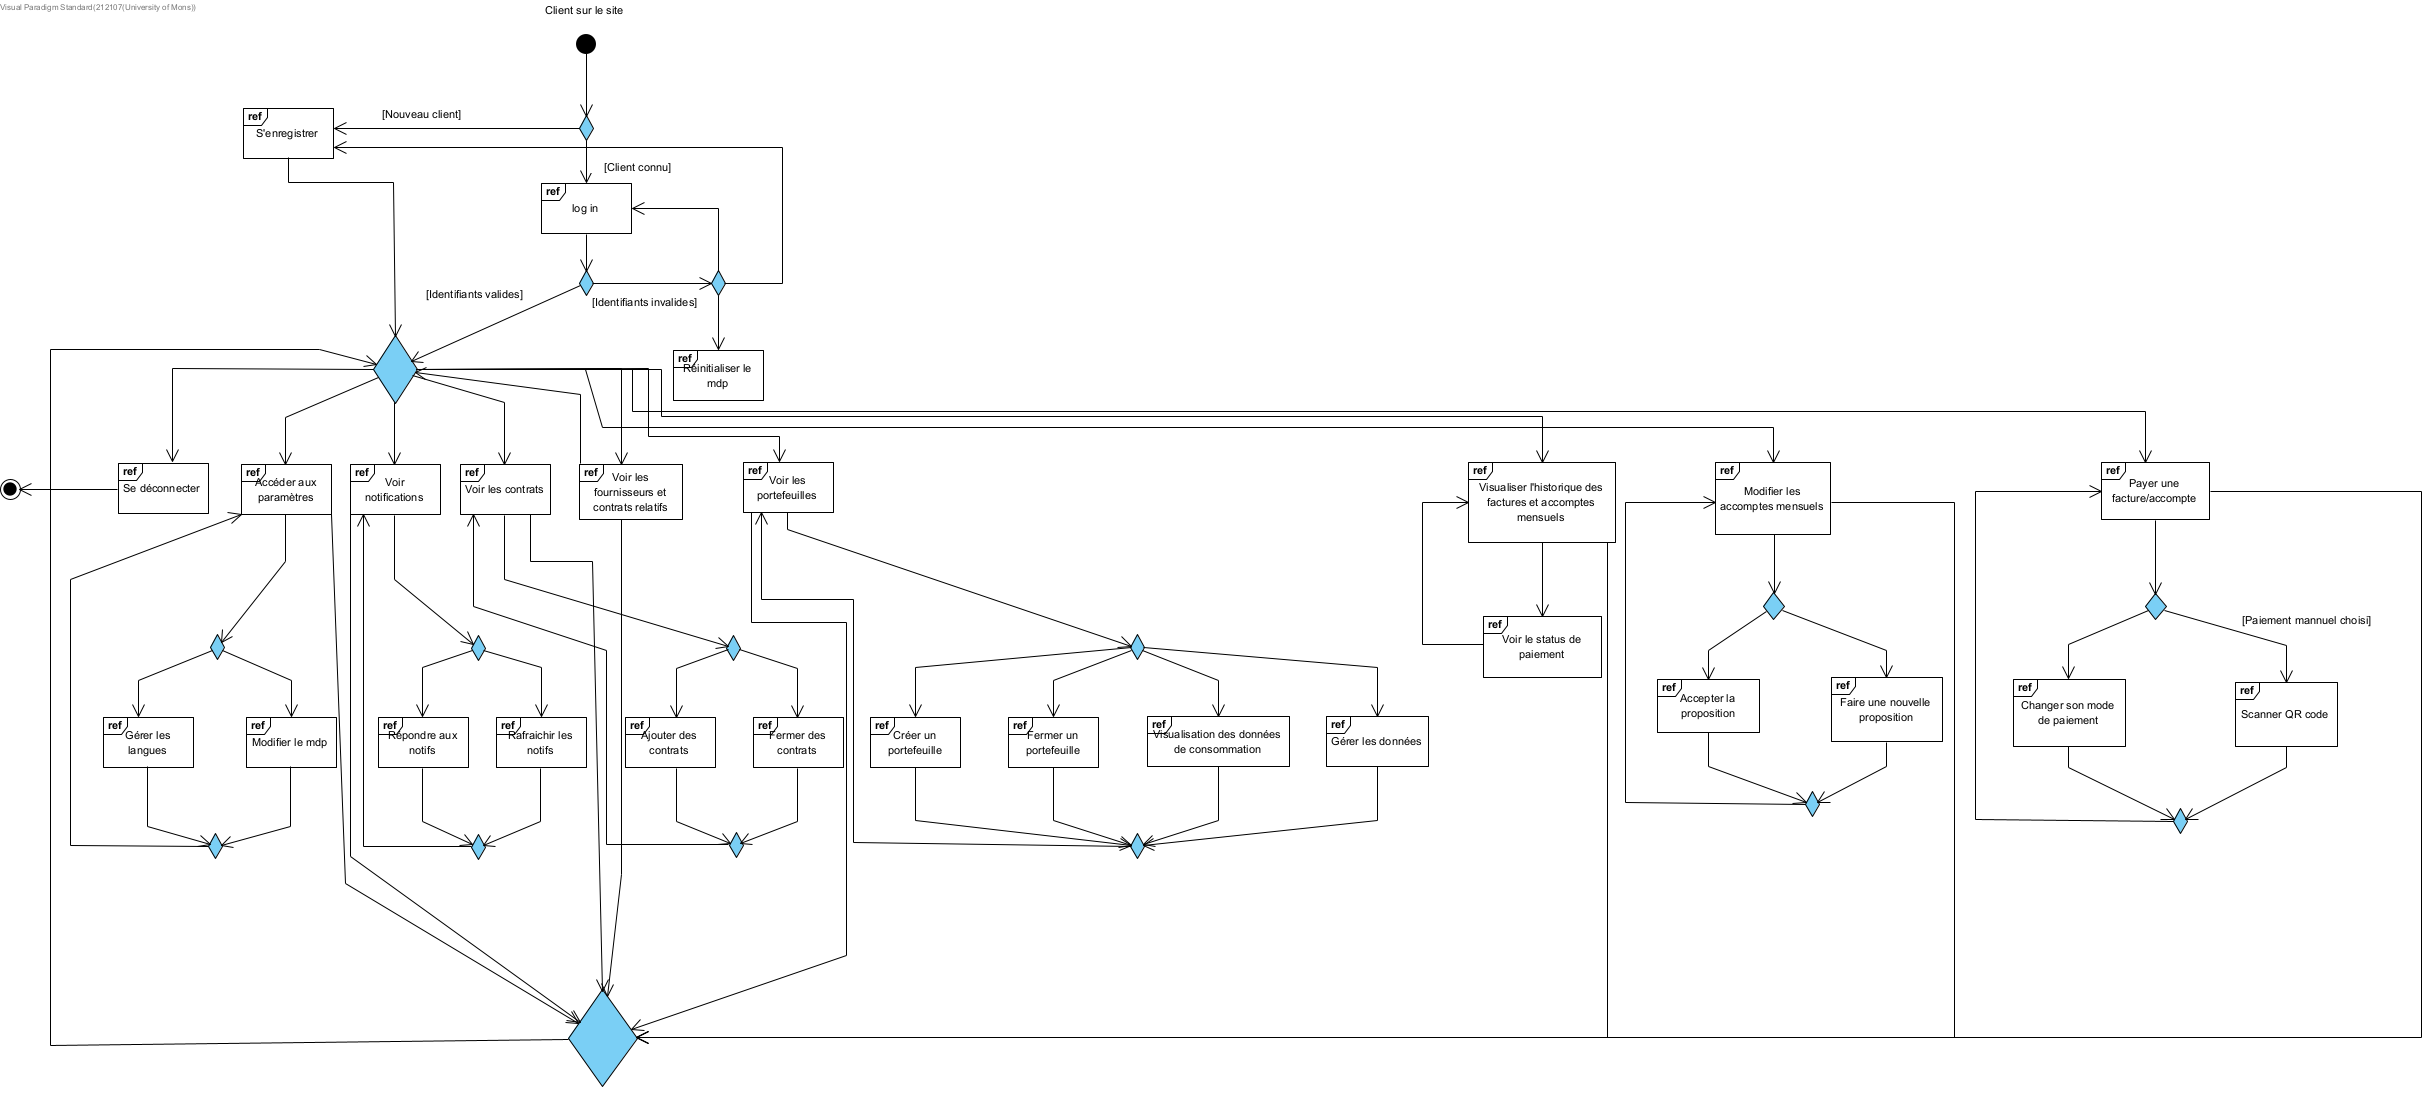
\includegraphics[width = 1\textwidth]{extension-maxime/interaction/img/interaction-extension.png}
\end{figure}

